\let\lesson\undefined
\newcommand{\lesson}{\phantomlesson{Bài 11: Ba định luật Newton về chuyển động}}
\chapter[Định luật II Newton]{Định luật II Newton}
\setcounter{section}{0}
\section{Lý thuyết}
\subsection{Định luật II Newton}
Gia tốc của vật có cùng hướng với lực tác dụng lên vật. Độ lớn của gia tốc tỉ lệ thuận với độ lớn của lực và tỉ lệ nghịch với khối lượng của vật.
\begin{equation*}
	\vec{a}=\dfrac{\vec F}{m},
\end{equation*}
trong đó:
\begin{itemize}
	\item $\vec F$ là lực tác dụng lên vật (N);
	\item m là khối lượng của vật (kg);
	\item $\vec a$ là gia tốc của vật ($\text{m/s}^2$).
\end{itemize}
Trong hệ SI, đơn vị của lực là $\si{\newton}$ (newton).\\
$$\SI{1}{\newton}=\SI{1}{\kilogram}\cdot\SI{1}{\meter/\second^2}$$
Trong trường hợp vật chịu tác dụng của nhiều lực thì lực $\vec{F}$ trong biểu thức là lực tổng hợp của tất cả các lực thành phần:
$$\vec{F}=\overrightarrow{F_1}+\overrightarrow{F_2}+\overrightarrow{F_3}+\dots$$
\subsection{Khối lượng và quán tính}
Khối lượng là đại lượng đặc trưng cho mức quán tính của vật. Vật có mức quán tính lớn hơn thì khối lượng lớn hơn và ngược lại. \\
Khối lượng là đại lượng vô hướng, dương, không đổi với mỗi vật \textit{(*)} và có tính chất cộng được.\\
\textit{(*) Chỉ đúng trong cơ học Newton (cơ học phi tương đối tính).}\\
\textbf{\textit{Ví dụ:}} Việc đẩy một chiếc xe máy đang bị chết máy để nó chuyển động sẽ dễ dàng hơn nhiều so với việc đẩy một chiếc ô tô chết máy dù tác dụng với cùng một lực. Vì xe ô tô có khối lượng lớn hơn nhiều so với xe máy, do đó quán tính của xe ô tô lớn hơn và khó thay đổi trạng thái chuyển động hơn.
\begin{center}
	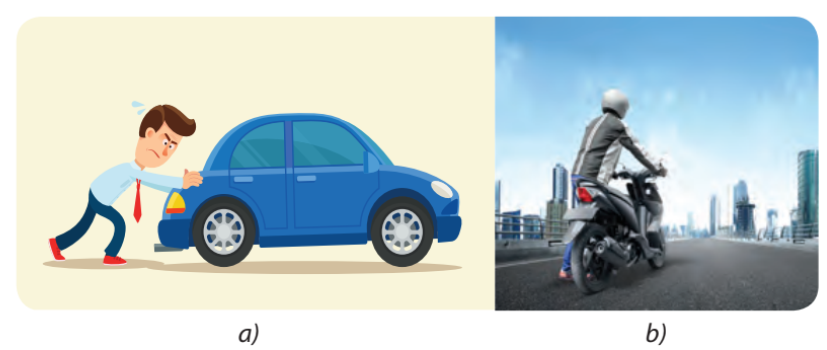
\includegraphics[width=0.5\linewidth]{../figs/VN10-2023-PH-TP016-1}
	\captionof{figure}{Một người đẩy \textit{a)} xe ô tô; \textit{b)} xe máy từ trạng thái nghỉ khi hai xe gặp sự cố.}
\end{center}
\subsection{Lực bằng nhau - Lực không bằng nhau}
\begin{itemize}
	\item \textbf{Hai lực bằng nhau:} khi lần lượt tác dụng vào cùng một vật sẽ gây ra lần lượt hai vectơ gia tốc bằng nhau (giống nhau về hướng và bằng nhau về độ lớn).
	\item \textbf{Hai lực không bằng nhau:} khi tác dụng lần lượt vào cùng một vật sẽ gây ra lần lượt hai vectơ gia tốc khác nhau (về hướng hoặc độ lớn).
\end{itemize}
\subsection{Lực cân bằng}
Nếu cho hai lực đồng thời tác dụng vào cùng một vật theo hướng ngược nhau, ta có hai trường hợp có thể xảy ra:
\begin{itemize}
	\item Vật đứng yên hoặc chuyển động thẳng đều. Hai lực này được gọi là \textbf{hai lực cân bằng}.
	\item Vật thu gia tốc và chuyển động theo hướng của lực có độ lớn lớn hơn. Hai lực này được gọi là \textbf{hai lực không cân bằng}.
\end{itemize}
\section{Mục tiêu bài học - Ví dụ minh họa}
\begin{dang}{Ghi nhớ định luật II Newton}
	\viduii{1}{Trong các cách viết công thức của định luật II Newton sau đây, cách viết nào đúng?
		\begin{mcq}(2)
			\item $\vec{F} = \dfrac{\vec{a}}{m}$.
			\item $\vec{a}=\dfrac{\vec{F}}{m}$. 
			\item $\vec{F} = - m\vec{a}$.
			\item $\vec{F} = ma.$
		\end{mcq}
		% Hung comment: bản ghi cũ sai: đáp án B F=ma không phải định luật 2 Newton, mà chỉ là một hệ quả được suy ra bằng cách biên đổi toán học công thức của định luật II Newton.	
	}
	{	\begin{center}
			\textbf{Hướng dẫn giải}
		\end{center}
		
		Gia tốc của một vật cùng hướng với lực tác dụng lên vật. Độ lớn của gia tốc tỉ lệ thuận với độ lớn của lực và tỉ lệ nghịch với khối lượng của vật.
		\begin{equation}
			\vec{a}=\dfrac{\vec F}{m},
		\end{equation}
		
		\textbf{Đáp án: B}
	}
	\viduii{1}{Chọn câu phát biểu đúng?
		\begin{mcq}
			\item Nếu không có lực tác dụng vào vật thì vật không chuyển động được. 
			\item Lực tác dụng luôn cùng hướng với hướng biến dạng. 
			\item Vật luôn chuyển động theo hướng của lực tác dụng. 
			\item Nếu vật chỉ chịu tác dụng của một lực khác không, thì vận tốc của vật sẽ bị thay đổi.
		\end{mcq}		
	}
	{	\begin{center}
			\textbf{Hướng dẫn giải}
		\end{center}
		
		Đáp án A: không có lực tác dụng thì vật vẫn có thể chuyển động thẳng đều nếu nó đang chuyển động thẳng đều. \\
		Đáp án B: Không có định luật nói về hướng của biến dạng dưới tác dụng của lực. \\
		Đáp án C: theo định luật II Newton, gia tốc luôn cùng hướng với lực tác dụng, chứ không phải vận tốc. \\
		Đáp án D: Nếu vật chỉ chịu tác dụng của một lực khác không thì vật thu gia tốc, đồng nghĩa rằng vận tốc của vật bị thay đổi. Đây là phát biểu đúng. 
		
		\textbf{Đáp án: D}
		%	Hung comment: phát biểu cũ của đáp án D: ``nếu có lực tác dụng lên vật thì vận tốc của vật bị thay đổi'' là chưa đúng. Vẫn có trường hợp vật chịu tác dụng của nhiều lực, nhưng hợp lực bằng không thì vật vẫn không thay đổi vận tốc. 	
	}
\end{dang}
\begin{dang}{Vận dụng được mối liên hệ $a=\dfrac{F}{m}$}
	\viduii{2}
	{Một quả bóng khối lượng $\SI{0.50}{\kilogram}$ đang nằm yên trên mặt đất. Một cầu thủ đá bóng với một lực $\SI{250}{\newton}$. Thời gian chân tác dụng vào bóng là $\SI{0.02}{\second}$. Quả bóng bay đi với tốc độ
		\begin{mcq}(2)
			\item $\SI{0.01}{\meter/\second}$.
			\item $\SI{0.10}{\meter/\second}$.
			\item $\SI{2.50}{\meter/\second}$.
			\item $\SI{10.00}{\meter/\second}$.
		\end{mcq}
	
}
{\begin{center}
		\textbf{Hướng dẫn giải}
	\end{center}
Gia tốc mà quả bóng thu được:
$$a=\dfrac{F}{m}=\dfrac{\SI{250}{\newton}}{\SI{0.50}{\kilogram}}=\SI{500}{\meter/\second^2}$$
Qủa bóng bay đi với tốc độ:
$$v=at=\left(\SI{500}{\meter/\second^2}\right)\cdot\left(\SI{0.02}{\second}\right)=\SI{10}{\meter/\second}.$$
}
\viduii{2}
{Dưới tác dụng của hợp lực $\SI{20}{\newton}$, một chiếc xe đồ chơi chuyển động với gia tốc $\SI{0.4}{\meter/\second^2}$. Dưới tác dụng của hợp lực $\SI{50}{\newton}$, chiếc xe sẽ chuyển động với gia tốc bao nhiêu?
}
{\begin{center}
		\textbf{Hướng dẫn giải}
	\end{center}
Vì khối lượng của vật là đại lượng không đổi nên
$$m=\dfrac{F_1}{a_1}=\dfrac{F_2}{a_2}\Rightarrow a_2=\dfrac{F_2}{F_1}\cdot a_1$$
$$\Rightarrow a_2=\dfrac{\left(\SI{50}{\newton}\right)}{\left(\SI{20}{\newton}\right)}\cdot\left(\SI{0.4}{\meter/\second^2}\right)=\SI{1}{\meter/\second^2}.$$
}
\viduii{3}
{Một xe bán tải khối lượng 2,5 tấn đang di chuyển trên cao tốc với tốc độ $\SI{90}{\kilo\meter/\hour}$. Các xe cần giữ khoảng cách an toàn so với xe phía trước $\SI{70}{\meter}$. Khi xe đi trước có sự cố và dừng lại đột ngột. Hãy xác định lực cản tối thiểu để xe bán tải có thể dừng lại an toàn.
}
{\begin{center}
		\textbf{Hướng dẫn giải}
	\end{center}
Đổi các đơn vị các dữ kiện trong đề bài theo hệ SI\\
$m=2,5 \text{tấn}=\SI{2.5E3}{\kilogram}$; $v_0=\SI{90}{\kilo\meter/\hour}=\SI{25}{\meter/\second}$.\\
Để xe bán tải dừng lại an toàn thì quãng đường xe chuyển động được kể từ lúc hãm phanh đến lúc dừng lại
$$s\le \SI{70}{\meter}$$
Gia tốc của xe trong quá trình hãm phanh
$$v^2-v^2_0=2as\Rightarrow a=\dfrac{-v^2_0}{2s}$$
$$\Rightarrow \left|a\right|=\dfrac{v^2_0}{2s}\ge \dfrac{\left(\SI{25}{\meter/\second}\right)^2}{2\cdot\left(\SI{70}{\meter}\right)}\approx\SI{4.46}{\meter/\second^2}$$
Độ lớn lực cản
$$\left|F\right|=m\cdot\left|a\right|\ge \left(\SI{2.5E3}{\kilogram}\right)\cdot\left(\SI{4.46}{\meter/\second^2}\right)=\SI{11150}{\newton}$$
Vậy lực cản tối thiểu để xe sau dừng lại an toàn là $\SI{11150}{\newton}$.
}
\end{dang}
